% Metódy inžinierskej práce

\documentclass[10pt,twoside,slovak,a4paper]{article}

\usepackage[slovak]{babel}
%\usepackage[T1]{fontenc}
\usepackage[IL2]{fontenc} % lepšia sadzba písmena Ľ než v T1
\usepackage[utf8]{inputenc}
\usepackage{graphicx}
\usepackage{url} % príkaz \url na formátovanie URL
\usepackage{hyperref} % odkazy v texte budú aktívne (pri niektorých triedach dokumentov spôsobuje posun textu)

\usepackage{cite}
%\usepackage{times}

\pagestyle{headings}

\title{Využitie Blockchainu v hernom svete
\thanks{Semestrálny projekt v predmete Metódy inžinierskej práce, ak. rok 2022/23, vedenie: Igor Stupavský}}

\author{Daniel Činčura\\[2pt]
	{\small Slovenská technická univerzita v Bratislave}\\
	{\small Fakulta informatiky a informačných technológií}\\
	{\small \texttt{xcincura@stuba.sk}}
	}

\date{\small 30. september 2022}



\begin{document}

\maketitle

\begin{abstract}
\ldots
\end{abstract}



\section{Úvod}

V súčastnosti implementáciu blockchainu nájdeme len v malom počte hier, ktoré pochádzajú hlavne od malých vývojárov. Najčastejšie nájdeme využitie blockchainu v metaverse, kde zohráva dôležitú rolu pri vývoji Webu 3.0, ktorý je predovšetkým o decentralizácii. Technológia blockchainu sa používa hlavne pri predaji herných predmetov. Tento predaj sa aj tak väčšinu času realizuje na webových stránkach a nie priamo v hre. Blockchaine v hernom priemysle má omnoho väčšie využitie, ako len predaj herných predmetov.
V tradičnej hernej architektúre, používatelia nevlastnia svoje herné dáta. Ak poskytovateľ hry ukončí svoje služby, používateľ príde o všetky dáta, čiže stratia všetok čas a úsilie ktoré hre obetovali. Vďaka smart kontraktom fungujúcich na blockchaine, môžeme vytvoriť herné servery a databázy, ktoré budú hráčom poskytovať herné dáta, ktoré budú skutočne vlastniť. Keď sa používatelia rozhodnú odísť, tieto údaje je možné jednoducho preniesť do novej hry. Všeobecná forma údajov, ktoré je možné prenášať medzi hrami, sa prezentuje ako „EXPTOKEN“, čo sú mince, ktoré užívatelia zarábajú, keď trávia čas v hre, a ktoré možno vymeniť za herné predmety a iné herné výhody.

Pridanie blockchainu do terajšej hernej architektúry sme bližšie opísali v časti 2. Dôležité komponenty blockchainu sú uvedené v časti 3. Hodnotenie používateľov sme bližšie opísali v sekcii 4. V sekcii 5 sme sa venovali experimentu. Záverečná poznámky a pohľady do budúcna prináša časť 6.




\section{Herná architektúra s použitím Blockchainu} \label{nejaka}

Ako sme už spomenuli blockchain by mal v hernom priemysle obrovské využitie. Viacero veľkých spoločností prišlo s nápadom integrovania tohto prvku do svojich hier. Existuje množstvo spôsobov integrácie blockchainu. V tejto časti sa pozrieme na implementáciu blockchainu do terajšej hernej architektúry, ale taktiež na architektúru v ktorej nie sú použité tradičné prvky. Architektúra obr.~\ref{f:rozhod} by mohla byť integrovaná s tradičnými hernými servermi. Hry by sa však mohli vyvíjať aj bez spoliehania sa na tradičnú štruktúru. Pre správnu komunikáciu medzi tradičnými hernými servermi a blockchain časťou potrebujeme časť s názvom framework wrapper. Táto architektúra umožňuje herným vývojárom úplne oddeliť hernú logiku od smart kontraktov.

\begin{figure}[h]
    \centering
    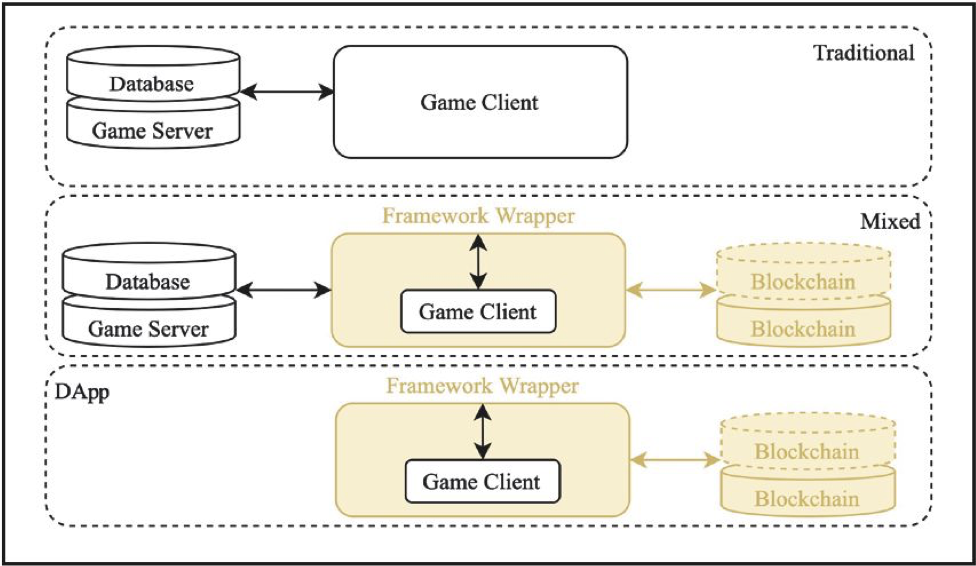
\includegraphics[scale=0.2]{blockchain_arch.png}
    \caption{Blockchain architektúra}\cite{Blockchain_architecture}  
    \label{fig:b-a}

\end{figure}





\section{Komponenty blockchainu} \label{komponenty}
Blockchainová časť našej architektúry je definovaná tak, že obsahuje tri hlavné komponenty. Sú to hráčsky komponent, blockchainový uzol a komponent pre vývojárov hier. Komponenty v našej architektúre medzi sebou komunikujú pomocou smart kontraktov.\cite{Blockchain_architecture}

\subsection{Komponent hráča} \label{komponenty:hrac}
Komponent hráča by fungoval ako komunikačný kanál medzi blockchainom a herným klientom. Ak chce hráč použiť blockchain na ukladanie herných dát (v našom modeli sme ich uložili ako EXPTOKEN), potrebuje sa zaregistrovať pomocou svojho súkromného kľúča a taktiež pridať aj adresu svojej peňaženky, na ktorú mu budú posielané tokeny.\cite{Blockchain_architecture}

\subsection{Blockchainový uzol} \label{komponenty:blockchain}
Komponent uzla blockchainu je klientsky uzol Etherea, ktorý sa používa na overovanie transakcií od klientov, pôsobí ako výbor na schvaľovanie nových hier, predchádzal by podvodom a udržiaval by herný štandard.\cite{Blockchain_architecture}

\subsection{Komponent vývojára} \label{komponenty:vyvojar}
Komponent vývojára predstavuje každého vývojára hier, ktorý by integroval architektúru do svojho vývojového kanála. V skutočnosti by to bol len smart kontrakt, ktorý by vývojári hier vložili do blockchainu.\cite{Blockchain_architecture}




\section{Vyplácanie hráčov} \label{vyplacanie}


\section{Herné tituly používajúce blockchain}\label{hry}
Už aj v súčastnosti existujú herné tituly, ktoré využívajú blockchain. Pri niektorých tituloch prišla implementácia blockchainu priskoro, čo sa potom odrazilo na jeho kvalite a funkčnosti. Medzi najznámejšie herné tituly využívajúce blockchain patria:
\begin{itemize}
    \item \textbf{Decentraland} - Táto hra využíva blockchain na vytvorenie virtuálneho a decentralizovaného sveta. V hre môžu používatelia objavovať svet, skupovať rôzne predmety a nehnuteľnosti.
    \item \textbf{Gods Unchained} - Gods Unchained je zberateľská kartová hra. Karty Gods Unchained sú digitálne aktíva, ktoré nemožno kopírovať ani upravovať bez súhlasu vlastníka, vďaka čomu sú jedinečné a hodnotné.
    \item \textbf{CryptoKitties} - Bola spustená v novembri 2017. Jedná sa o jednu z prvých hier, ktoré využívali blockchain. V súčasnosti sa stala jednou z najpopulárnejších hier postavených na Ethereu. Hlavným cieľom hry je vytvoriť novú generáciu mačiatok s jedinečnými vlastnosťami, aby sa maximalizovala ich hodnota.
\end{itemize}

\section{Záver a pohľady do budúcna} \label{zaver}
Blockchain má v budúcnosti herného priemyslu určite dôležité miesto. Všetko záleží od toho ako ho herná komunita akceptuje. Vykonalo sa už viacero experimentov, ktoré ukazujú pozitívnu odozvu hráčov na implementáciu blockchainu do herného sveta. Okrem toho, ako sa technológia neustále vyvíja a čoraz viac sa používa, môžeme očakávať, že v hrách uvidíme viac funkcií a aplikácií pre Blockchain. Vrátane rýchlejších a bezpečnejších transakcií, decentralizovaných platforiem pre virtuálne svety a nových foriem digitálnych aktív.  



% týmto sa generuje zoznam literatúry z obsahu súboru literatura.bib podľa toho, na čo sa v článku odkazujete
\bibliography{literatura}
\bibliographystyle{abbrv} % prípadne alpha, abbrv alebo hociktorý iný
\end{document}